\chapter{TOOL AND TECHNOLOGY}

This chapter presents the tools, libraries, and technologies used in the development and implementation of the proposed \textbf{\textit{KFCProcedure}} and \textbf{\textit{GradientCOBRA}} frameworks. The system is fully implemented in Python and relies on several scientific computing and machine learning libraries to support data processing, model training, and evaluation.

\section{Programming Language}

\begin{figure}[H]
    \centering
    
\includegraphics[width=0.25\textwidth]{figures/tools/python.png}
    \caption{Python Programming Language}
    \label{fig:python}
\end{figure}

The entire system is implemented using Python, which is widely used in machine learning research due to its simplicity, readability, and extensive ecosystem of scientific libraries. Python provides strong support for numerical computation, data manipulation, and machine learning model development, making it suitable for implementing both KFCProcedure and GradientCOBRA frameworks.

\section{Machine Learning Libraries}

The proposed system is implemented using a set of machine learning and scientific computing libraries in Python. These libraries provide the fundamental building blocks for data processing, model development, optimization, and evaluation in both KFCProcedure and GradientCOBRA frameworks. Each library plays a specific role in ensuring computational efficiency, modularity, and scalability of the system.

\subsection{Numpy}
\begin{figure}[H]
    \centering
    
\includegraphics[width=0.25\textwidth]{figures/tools/numpy.png}
    \caption{NumPy in Scientific Computing}
    \label{fig:numpy}
\end{figure}

NumPy is the core numerical computing library used in the system. It provides efficient support for multi-dimensional arrays, linear algebra operations, and vectorized computations. In the proposed frameworks, NumPy is primarily used for handling dataset representations, prediction matrices, distance computations, and mathematical transformations required in both clustering and aggregation processes.

\subsection{Scikit Learn}
\begin{figure}[H]
    \centering
    
\includegraphics[width=0.25\textwidth]{figures/tools/sklearn.png}
    \caption{Scikit-Learn Machine Learning Framework}
    \label{fig:sklearn}
\end{figure}

Scikit-learn is used as the primary machine learning library for implementing base estimators, preprocessing utilities, and evaluation metrics. It provides a wide range of regression and classification models that can be integrated into both KFCProcedure and GradientCOBRA frameworks. Additionally, it supports data splitting, scaling, and performance evaluation, which are essential for experimental validation.

\subsection{Scipy}

\begin{figure}[H]
    \centering
    
\includegraphics[width=0.25\textwidth]{figures/tools/scipy.png}
    \caption{SciPy Scientific Computing Library}
    \label{fig:scipy}
\end{figure}

SciPy is utilized for advanced mathematical operations and optimization-related computations. It supports statistical functions, numerical integration, and optimization routines that are useful in the GradientCOBRA framework, particularly in kernel transformations and loss-related computations.

\subsection{Joblib}

\begin{figure}[H]
    \centering
    
\includegraphics[width=0.25\textwidth]{figures/tools/joblib.png}
    \caption{Joblib Parallel Processing Utility}
    \label{fig:joblib}
\end{figure}

Joblib is used for model persistence and efficient computation through parallel processing. In the proposed system, it supports saving trained models and improving execution efficiency when handling multiple estimators or cluster-wise models in KFCProcedure.

\subsection{Summary of Machine Learning Libraries}

Overall, these libraries form the computational backbone of the proposed system. NumPy provides numerical efficiency, scikit-learn enables machine learning modeling, SciPy supports mathematical optimization, and Joblib enhances performance and scalability. The integration of these libraries ensures that both KFCProcedure and GradientCOBRA can be implemented in a modular, efficient, and reproducible manner.

\section{Development Environment}

The development environment defines the software tools and platforms used to implement, test, and execute the proposed KFCProcedure and GradientCOBRA frameworks. A well-structured development environment is essential for ensuring reproducibility, efficient debugging, and smooth experimentation during model development. In this study, the system is developed using Python-based tools combined with modern code editors and notebook environments.

The primary development environment includes an integrated development environment (IDE) for code writing and debugging, as well as an interactive notebook interface for experimentation and visualization. These tools support iterative development, allowing rapid testing of clustering methods, predictive models, and optimization strategies. In addition, version control tools are used to manage code changes and maintain project consistency throughout development.

\subsection{Visual Studio Code}

\begin{figure}[H]
    \centering
    
\includegraphics[width=0.25\textwidth]{figures/tools/vscode.png}
    \caption{Integrated Development Environment}
    \label{fig:vscode}
\end{figure}

Visual Studio Code is used as the main integrated development environment for implementing the proposed system. These IDEs provide features such as syntax highlighting, debugging tools, code navigation, and plugin support, which significantly improve development efficiency. They are particularly useful for managing the modular structure of both KFCProcedure and GradientCOBRA packages.

\subsection{Jupyter Notebook}

\begin{figure}[H]
    \centering
    \includegraphics[width=0.25\textwidth]{figures/tools/jupyter.png}
    \caption{Jupyter Notebook Environment}
    \label{fig:jupyter}
\end{figure}

Jupyter Notebook is used for experimental development, testing, and visualization of intermediate results. It allows step-by-step execution of code, making it suitable for validating clustering outputs, model predictions, and optimization behavior. This environment is especially useful for comparing different configurations of GradientCOBRA and KFCProcedure in an interactive manner.

\subsection{Version Control System (Git/GitHub)}

\begin{figure}[H]
    \centering
    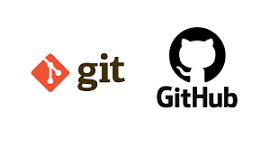
\includegraphics[width=0.5\textwidth]{figures/tools/git.png}
    \caption{Git and GitHub Workflow}
    \label{fig:git}
\end{figure}

Git and GitHub are used for version control and source code management throughout the development of the system. Git is used locally to track changes in the codebase, manage different versions of the project, and enable rollback to previous states when necessary. GitHub is used as a remote repository hosting platform to store the project, maintain backups, and facilitate collaboration and version synchronization. This combination ensures that the development of both KFCProcedure and GradientCOBRA frameworks is well-organized, traceable, and reproducible.

\subsection{Summary of Development Environment}

Overall, the development environment provides a robust and efficient setup for implementing the proposed system. The combination of IDEs for structured coding, Jupyter Notebook for experimentation, and Git for version control ensures a reliable workflow for developing, testing, and maintaining both machine learning frameworks. This environment supports reproducibility and facilitates systematic experimentation across all stages of the project.

\section{Visualization Tools}

Visualization tools are used in the proposed system to analyze, interpret, and present experimental results in a clear and meaningful way. Since both KFCProcedure and GradientCOBRA generate numerical outputs such as predictions, errors, and performance metrics, visualization is essential for understanding model behavior and comparing results across different configurations.

The visualization process mainly focuses on displaying model performance, error trends, and comparative analysis between different predictive approaches. These visual representations help in identifying patterns such as convergence behavior in optimization, differences between predicted and actual values, and overall model stability. In addition, visualization plays a key role in evaluating the effectiveness of clustering and aggregation mechanisms used in the proposed frameworks.

\subsection{Matplotlib}

\begin{figure}[H]
    \centering
    
\includegraphics[width=0.5\textwidth]{figures/tools/matplotlib.png}
    \caption{Matplotlib Visualization Library}
    \label{fig:matplotlib}
\end{figure}

Matplotlib is the primary library used for creating static visualizations such as line plots, scatter plots, and bar charts. It is widely used for plotting evaluation metrics like MAE, RMSE, and loss curves during training and optimization processes. In this study, Matplotlib is used to visualize model performance comparisons between KFCProcedure, GradientCOBRA, and any baseline methods.

\subsection{Seaborn}

\begin{figure}[H]
    \centering
    
\includegraphics[width=0.5\textwidth]{figures/tools/seaborn.png}
    \caption{Seaborn Statistical Data Visualization Library}
    \label{fig:seaborn}
\end{figure}

Seaborn is used for advanced statistical data visualization, providing more visually appealing and informative graphs compared to basic plotting tools. It is particularly useful for heatmaps, distribution plots, and correlation analysis between features and predictions. In the proposed system, Seaborn helps in understanding relationships between variables and evaluating model behavior across datasets.

\subsection{Summary of Visualization Tools}

Overall, visualization tools play an important role in interpreting experimental results and validating the performance of the proposed frameworks. Matplotlib provides flexible and detailed plotting capabilities for performance metrics, while Seaborn enhances statistical analysis through advanced visualization techniques. Together, these tools support a clear and comprehensive understanding of model behavior and experimental outcomes.

